\documentclass[twoside]{book}

% Packages required by doxygen
\usepackage{calc}
\usepackage{doxygen}
\usepackage{graphicx}
\usepackage[utf8]{inputenc}
\usepackage{makeidx}
\usepackage{multicol}
\usepackage{multirow}
\usepackage{fixltx2e}
\PassOptionsToPackage{warn}{textcomp}
\usepackage{textcomp}
\usepackage[nointegrals]{wasysym}
\usepackage[table]{xcolor}

% Font selection
\usepackage[T1]{fontenc}
\usepackage{mathptmx}
\usepackage[scaled=.90]{helvet}
\usepackage{courier}
\usepackage{amssymb}
\usepackage{sectsty}
\renewcommand{\familydefault}{\sfdefault}
\allsectionsfont{%
  \fontseries{bc}\selectfont%
  \color{darkgray}%
}
\renewcommand{\DoxyLabelFont}{%
  \fontseries{bc}\selectfont%
  \color{darkgray}%
}
\newcommand{\+}{\discretionary{\mbox{\scriptsize$\hookleftarrow$}}{}{}}

% Page & text layout
\usepackage{geometry}
\geometry{%
  a4paper,%
  top=2.5cm,%
  bottom=2.5cm,%
  left=2.5cm,%
  right=2.5cm%
}
\tolerance=750
\hfuzz=15pt
\hbadness=750
\setlength{\emergencystretch}{15pt}
\setlength{\parindent}{0cm}
\setlength{\parskip}{0.2cm}
\makeatletter
\renewcommand{\paragraph}{%
  \@startsection{paragraph}{4}{0ex}{-1.0ex}{1.0ex}{%
    \normalfont\normalsize\bfseries\SS@parafont%
  }%
}
\renewcommand{\subparagraph}{%
  \@startsection{subparagraph}{5}{0ex}{-1.0ex}{1.0ex}{%
    \normalfont\normalsize\bfseries\SS@subparafont%
  }%
}
\makeatother

% Headers & footers
\usepackage{fancyhdr}
\pagestyle{fancyplain}
\fancyhead[LE]{\fancyplain{}{\bfseries\thepage}}
\fancyhead[CE]{\fancyplain{}{}}
\fancyhead[RE]{\fancyplain{}{\bfseries\leftmark}}
\fancyhead[LO]{\fancyplain{}{\bfseries\rightmark}}
\fancyhead[CO]{\fancyplain{}{}}
\fancyhead[RO]{\fancyplain{}{\bfseries\thepage}}
\fancyfoot[LE]{\fancyplain{}{}}
\fancyfoot[CE]{\fancyplain{}{}}
\fancyfoot[RE]{\fancyplain{}{\bfseries\scriptsize Generated on Wed Jun 4 2014 20\+:39\+:55 for Proeve van Bekwaamheid by Doxygen }}
\fancyfoot[LO]{\fancyplain{}{\bfseries\scriptsize Generated on Wed Jun 4 2014 20\+:39\+:55 for Proeve van Bekwaamheid by Doxygen }}
\fancyfoot[CO]{\fancyplain{}{}}
\fancyfoot[RO]{\fancyplain{}{}}
\renewcommand{\footrulewidth}{0.4pt}
\renewcommand{\chaptermark}[1]{%
  \markboth{#1}{}%
}
\renewcommand{\sectionmark}[1]{%
  \markright{\thesection\ #1}%
}

% Indices & bibliography
\usepackage{natbib}
\usepackage[titles]{tocloft}
\setcounter{tocdepth}{3}
\setcounter{secnumdepth}{5}
\makeindex

% Hyperlinks (required, but should be loaded last)
\usepackage{ifpdf}
\ifpdf
  \usepackage[pdftex,pagebackref=true]{hyperref}
\else
  \usepackage[ps2pdf,pagebackref=true]{hyperref}
\fi
\hypersetup{%
  colorlinks=true,%
  linkcolor=blue,%
  citecolor=blue,%
  unicode%
}

% Custom commands
\newcommand{\clearemptydoublepage}{%
  \newpage{\pagestyle{empty}\cleardoublepage}%
}


%===== C O N T E N T S =====

\begin{document}

% Titlepage & ToC
\hypersetup{pageanchor=false,
             bookmarks=true,
             bookmarksnumbered=true,
             pdfencoding=unicode
            }
\pagenumbering{roman}
\begin{titlepage}
\vspace*{7cm}
\begin{center}%
{\Large Proeve van Bekwaamheid \\[1ex]\large 1.\+1 }\\
\vspace*{1cm}
{\large Generated by Doxygen 1.8.7}\\
\vspace*{0.5cm}
{\small Wed Jun 4 2014 20:39:55}\\
\end{center}
\end{titlepage}
\clearemptydoublepage
\tableofcontents
\clearemptydoublepage
\pagenumbering{arabic}
\hypersetup{pageanchor=true}

%--- Begin generated contents ---
\chapter{Hierarchical Index}
\section{Class Hierarchy}
This inheritance list is sorted roughly, but not completely, alphabetically\+:\begin{DoxyCompactList}
\item Editor\begin{DoxyCompactList}
\item \contentsline{section}{Drop\+Borders\+Helper}{\pageref{class_drop_borders_helper}}{}
\item \contentsline{section}{Game\+Config\+Helper}{\pageref{class_game_config_helper}}{}
\end{DoxyCompactList}
\item Mono\+Behaviour\begin{DoxyCompactList}
\item \contentsline{section}{Accelerometer\+Input}{\pageref{class_accelerometer_input}}{}
\item \contentsline{section}{Animated\+Billboard}{\pageref{class_animated_billboard}}{}
\item \contentsline{section}{Application\+Exit}{\pageref{class_application_exit}}{}
\item \contentsline{section}{Block\+Recycler}{\pageref{class_block_recycler}}{}
\item \contentsline{section}{Block\+Transparency}{\pageref{class_block_transparency}}{}
\item \contentsline{section}{button\+Color}{\pageref{classbutton_color}}{}
\item \contentsline{section}{Drop\+Block}{\pageref{class_drop_block}}{}
\item \contentsline{section}{Drop\+Borders}{\pageref{class_drop_borders}}{}
\item \contentsline{section}{Finish\+Trigger}{\pageref{class_finish_trigger}}{}
\item \contentsline{section}{Follow\+Player}{\pageref{class_follow_player}}{}
\item \contentsline{section}{Game\+Config}{\pageref{class_game_config}}{}
\item \contentsline{section}{go\+To\+Menu}{\pageref{classgo_to_menu}}{}
\item \contentsline{section}{High\+Score\+G\+U\+I}{\pageref{class_high_score_g_u_i}}{}
\item \contentsline{section}{Instantiate\+Game}{\pageref{class_instantiate_game}}{}
\item \contentsline{section}{Menu\+Script}{\pageref{class_menu_script}}{}
\item \contentsline{section}{Pause\+Conditions}{\pageref{class_pause_conditions}}{}
\item \contentsline{section}{Pickup\+Coin}{\pageref{class_pickup_coin}}{}
\item \contentsline{section}{Reset\+Player}{\pageref{class_reset_player}}{}
\item \contentsline{section}{Rotate\+G\+U\+I}{\pageref{class_rotate_g_u_i}}{}
\item \contentsline{section}{Scale\+In\+Game\+G\+U\+I}{\pageref{class_scale_in_game_g_u_i}}{}
\item \contentsline{section}{Score\+Counter}{\pageref{class_score_counter}}{}
\item \contentsline{section}{Spawn\+Point}{\pageref{class_spawn_point}}{}
\item \contentsline{section}{tutorial\+Pressed}{\pageref{classtutorial_pressed}}{}
\item \contentsline{section}{U\+I\+Level\+Select}{\pageref{class_u_i_level_select}}{}
\item \contentsline{section}{Water\+Transparency}{\pageref{class_water_transparency}}{}
\item \contentsline{section}{Water\+Trigger}{\pageref{class_water_trigger}}{}
\item \contentsline{section}{win\+Now}{\pageref{classwin_now}}{}
\item \contentsline{section}{Won\+Screen}{\pageref{class_won_screen}}{}
\end{DoxyCompactList}
\end{DoxyCompactList}

\chapter{Class Index}
\section{Class List}
Here are the classes, structs, unions and interfaces with brief descriptions\+:\begin{DoxyCompactList}
\item\contentsline{section}{\hyperlink{class_accelerometer_input}{Accelerometer\+Input} \\*This component controls the obj\+\_\+\+Player by measuring the accelerometer input if played on Android otherwise this function controls obj\+\_\+\+Player via W A S D and arrow keys. }{\pageref{class_accelerometer_input}}{}
\item\contentsline{section}{\hyperlink{class_animated_billboard}{Animated\+Billboard} \\*This component animates a given texture via U\+V coordinates. }{\pageref{class_animated_billboard}}{}
\item\contentsline{section}{\hyperlink{class_application_exit}{Application\+Exit} \\*This component allows the application to exit on any platform. }{\pageref{class_application_exit}}{}
\item\contentsline{section}{\hyperlink{class_block_recycler}{Block\+Recycler} \\*This component recycles objects by placing them 1000f units away on the Z-\/axis. }{\pageref{class_block_recycler}}{}
\item\contentsline{section}{\hyperlink{class_block_transparency}{Block\+Transparency} \\*This component allows for transparent transition of a Game\+Object if some other collider is nearby. In this case the Player. }{\pageref{class_block_transparency}}{}
\item\contentsline{section}{\hyperlink{class_drop_block}{Drop\+Block} \\*Component used to ease a levelpart downwards. Controlled in the editor by Drop\+Block\+Helper }{\pageref{class_drop_block}}{}
\item\contentsline{section}{\hyperlink{class_drop_borders}{Drop\+Borders} \\*This component lowers or raises the borders as one object. This component is dependent on \hyperlink{class_drop_block}{Drop\+Block}'s interaction with the player. }{\pageref{class_drop_borders}}{}
\item\contentsline{section}{\hyperlink{class_follow_player}{Follow\+Player} \\*This component ensures the Camera follows the player. The player\+Object is checked for an active instane as well. }{\pageref{class_follow_player}}{}
\item\contentsline{section}{\hyperlink{class_game_config}{Game\+Config} \\*Configuration for the game. For use with Get\+Component$<$$>$(); Controlled in the editor by Game\+Config\+Helper }{\pageref{class_game_config}}{}
\item\contentsline{section}{\hyperlink{class_high_score_g_u_i}{High\+Score\+G\+U\+I} }{\pageref{class_high_score_g_u_i}}{}
\item\contentsline{section}{\hyperlink{class_instantiate_game}{Instantiate\+Game} \\*This component is responsible for loading and instantiating objects needed for the game. 
\begin{DoxyParams}{Parameters}
{\em player} & The prefab/\+Game\+Object controlled by the player\\
\hline
{\em level} & The switchable level, switchable by setting 'level\+Name'\\
\hline
{\em playing\+Field\+Volume} & The box collider to aid in 'respawning' the player by setting the proper\\
\hline
\end{DoxyParams}
}{\pageref{class_instantiate_game}}{}
\item\contentsline{section}{\hyperlink{class_pause_conditions}{Pause\+Conditions} }{\pageref{class_pause_conditions}}{}
\item\contentsline{section}{\hyperlink{class_pickup_coin}{Pickup\+Coin} }{\pageref{class_pickup_coin}}{}
\item\contentsline{section}{\hyperlink{class_reset_player}{Reset\+Player} \\*This component ensures the level resets the player. }{\pageref{class_reset_player}}{}
\item\contentsline{section}{\hyperlink{class_rotate_g_u_i}{Rotate\+G\+U\+I} }{\pageref{class_rotate_g_u_i}}{}
\item\contentsline{section}{\hyperlink{class_scale_in_game_g_u_i}{Scale\+In\+Game\+G\+U\+I} }{\pageref{class_scale_in_game_g_u_i}}{}
\item\contentsline{section}{\hyperlink{class_score_counter}{Score\+Counter} }{\pageref{class_score_counter}}{}
\item\contentsline{section}{\hyperlink{class_spawn_point}{Spawn\+Point} \\*Helper class, to store the \hyperlink{class_spawn_point}{Spawn\+Point}. For use with Get\+Component$<$$>$(); }{\pageref{class_spawn_point}}{}
\item\contentsline{section}{\hyperlink{class_u_i_level_select}{U\+I\+Level\+Select} }{\pageref{class_u_i_level_select}}{}
\end{DoxyCompactList}

\chapter{Class Documentation}
\hypertarget{class_accelerometer_input}{\section{Accelerometer\+Input Class Reference}
\label{class_accelerometer_input}\index{Accelerometer\+Input@{Accelerometer\+Input}}
}


This component controls the obj\+\_\+\+Player by measuring the accelerometer input if played on Android otherwise this function controls obj\+\_\+\+Player via W A S D and arrow keys.  


Inheritance diagram for Accelerometer\+Input\+:\begin{figure}[H]
\begin{center}
\leavevmode
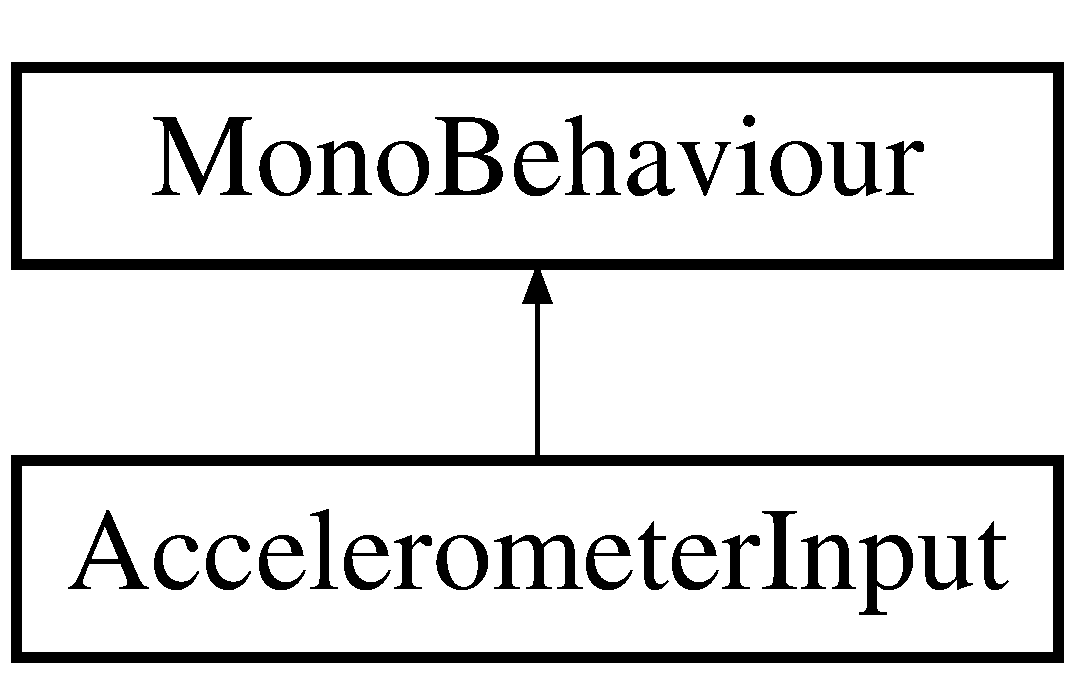
\includegraphics[height=2.000000cm]{class_accelerometer_input}
\end{center}
\end{figure}


\subsection{Detailed Description}
This component controls the obj\+\_\+\+Player by measuring the accelerometer input if played on Android otherwise this function controls obj\+\_\+\+Player via W A S D and arrow keys. 



Definition at line 9 of file Accelerometer\+Input.\+cs.



The documentation for this class was generated from the following file\+:\begin{DoxyCompactItemize}
\item 
Assets/\+Scripts/\+Player\+Scripts/Accelerometer\+Input.\+cs\end{DoxyCompactItemize}

\hypertarget{class_animated_billboard}{\section{Animated\+Billboard Class Reference}
\label{class_animated_billboard}\index{Animated\+Billboard@{Animated\+Billboard}}
}


This component animates a given texture via U\+V coordinates.  


Inheritance diagram for Animated\+Billboard\+:\begin{figure}[H]
\begin{center}
\leavevmode
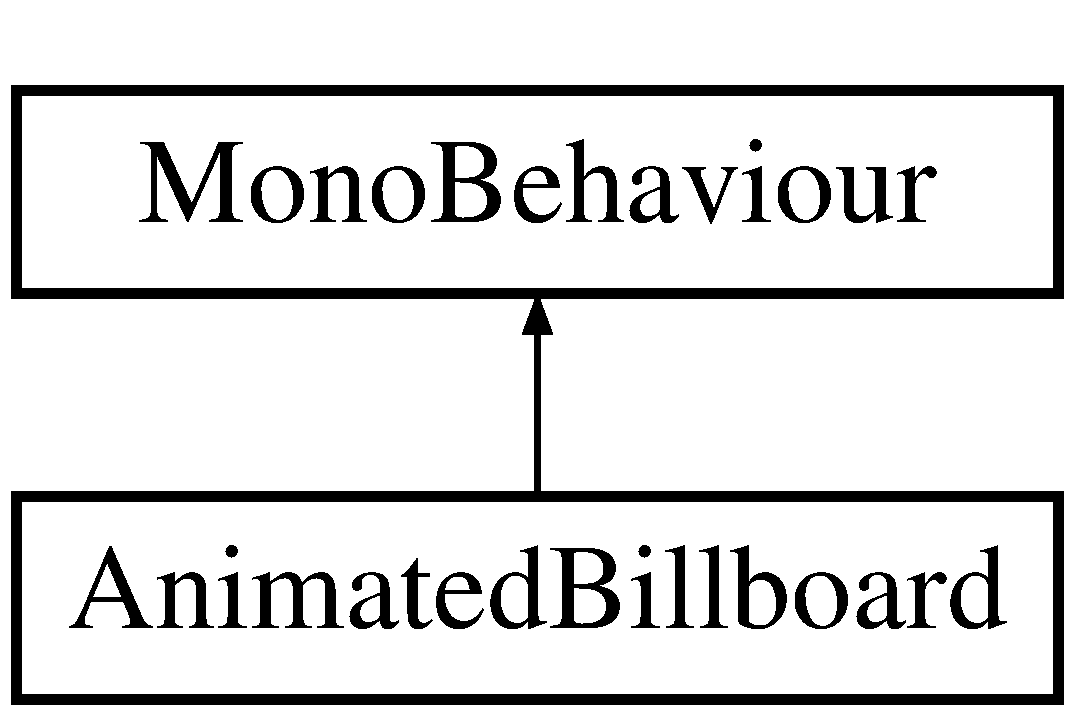
\includegraphics[height=2.000000cm]{class_animated_billboard}
\end{center}
\end{figure}
\subsection*{Public Attributes}
\begin{DoxyCompactItemize}
\item 
\hypertarget{class_animated_billboard_a10edd130c334ea6aa0444c3338e65d8c}{int {\bfseries \+\_\+uv\+Tie\+X} = 1}\label{class_animated_billboard_a10edd130c334ea6aa0444c3338e65d8c}

\item 
\hypertarget{class_animated_billboard_a059abeaabfc49d03b412947b44397bc7}{int {\bfseries \+\_\+uv\+Tie\+Y} = 1}\label{class_animated_billboard_a059abeaabfc49d03b412947b44397bc7}

\item 
\hypertarget{class_animated_billboard_a521d074d952fea3d579e4a8b40ac91ea}{int {\bfseries \+\_\+fps} = 10}\label{class_animated_billboard_a521d074d952fea3d579e4a8b40ac91ea}

\end{DoxyCompactItemize}


\subsection{Detailed Description}
This component animates a given texture via U\+V coordinates. 



Definition at line 6 of file Animated\+Billboard.\+cs.



The documentation for this class was generated from the following file\+:\begin{DoxyCompactItemize}
\item 
Assets/\+Scripts/Animated\+Billboard.\+cs\end{DoxyCompactItemize}

\hypertarget{class_application_exit}{\section{Application\+Exit Class Reference}
\label{class_application_exit}\index{Application\+Exit@{Application\+Exit}}
}


This component allows the application to exit on any platform.  


Inheritance diagram for Application\+Exit\+:\begin{figure}[H]
\begin{center}
\leavevmode
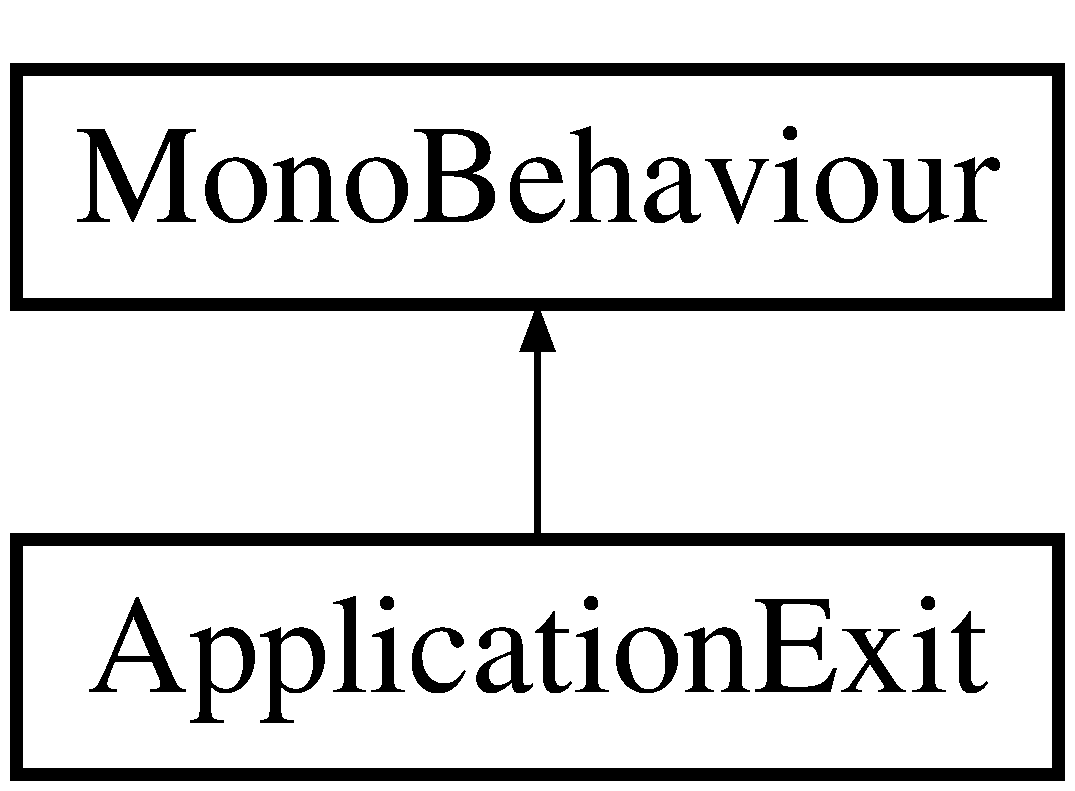
\includegraphics[height=2.000000cm]{class_application_exit}
\end{center}
\end{figure}


\subsection{Detailed Description}
This component allows the application to exit on any platform. 



Definition at line 7 of file Application\+Exit.\+cs.



The documentation for this class was generated from the following file\+:\begin{DoxyCompactItemize}
\item 
Assets/\+Scripts/Application\+Exit.\+cs\end{DoxyCompactItemize}

\hypertarget{class_block_recycler}{\section{Block\+Recycler Class Reference}
\label{class_block_recycler}\index{Block\+Recycler@{Block\+Recycler}}
}


This component recycles objects by placing them 1000f units away on the Z-\/axis.  


Inheritance diagram for Block\+Recycler\+:\begin{figure}[H]
\begin{center}
\leavevmode
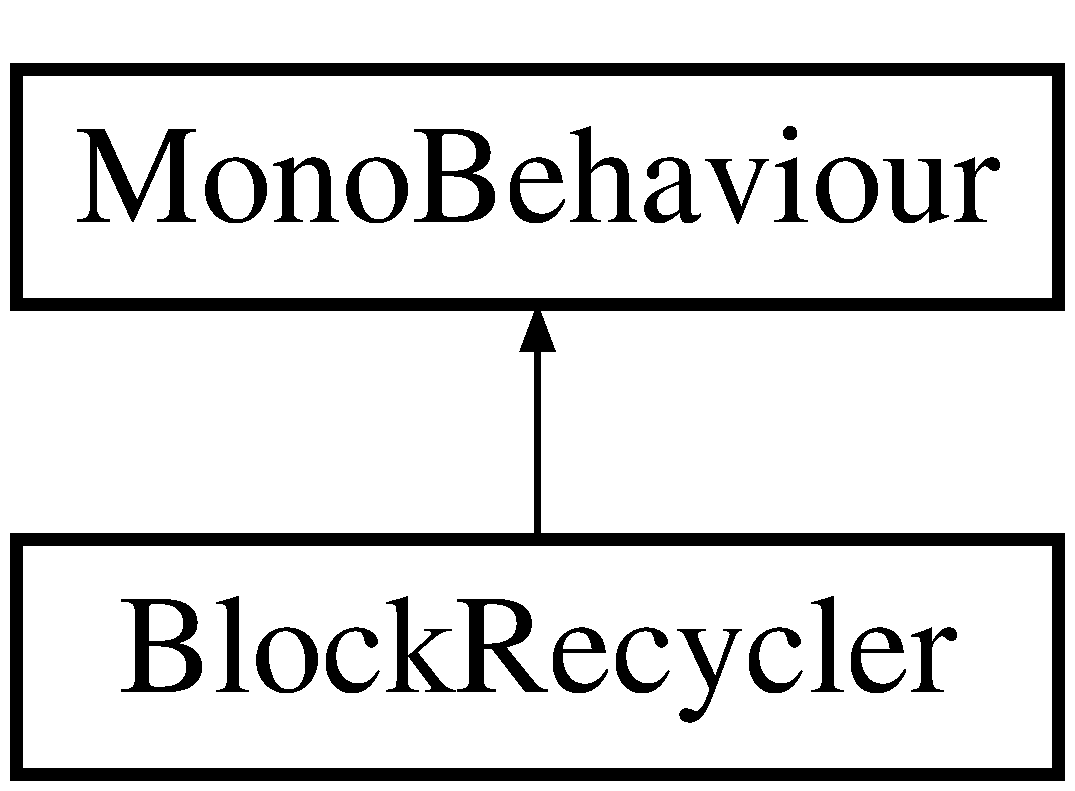
\includegraphics[height=2.000000cm]{class_block_recycler}
\end{center}
\end{figure}


\subsection{Detailed Description}
This component recycles objects by placing them 1000f units away on the Z-\/axis. 



Definition at line 7 of file Block\+Recycler.\+cs.



The documentation for this class was generated from the following file\+:\begin{DoxyCompactItemize}
\item 
Assets/\+Scripts/\+Level\+Scripts/Block\+Recycler.\+cs\end{DoxyCompactItemize}

\hypertarget{class_block_transparency}{\section{Block\+Transparency Class Reference}
\label{class_block_transparency}\index{Block\+Transparency@{Block\+Transparency}}
}


This component allows for transparent transition of a Game\+Object if some other collider is nearby. In this case the Player.  


Inheritance diagram for Block\+Transparency\+:\begin{figure}[H]
\begin{center}
\leavevmode
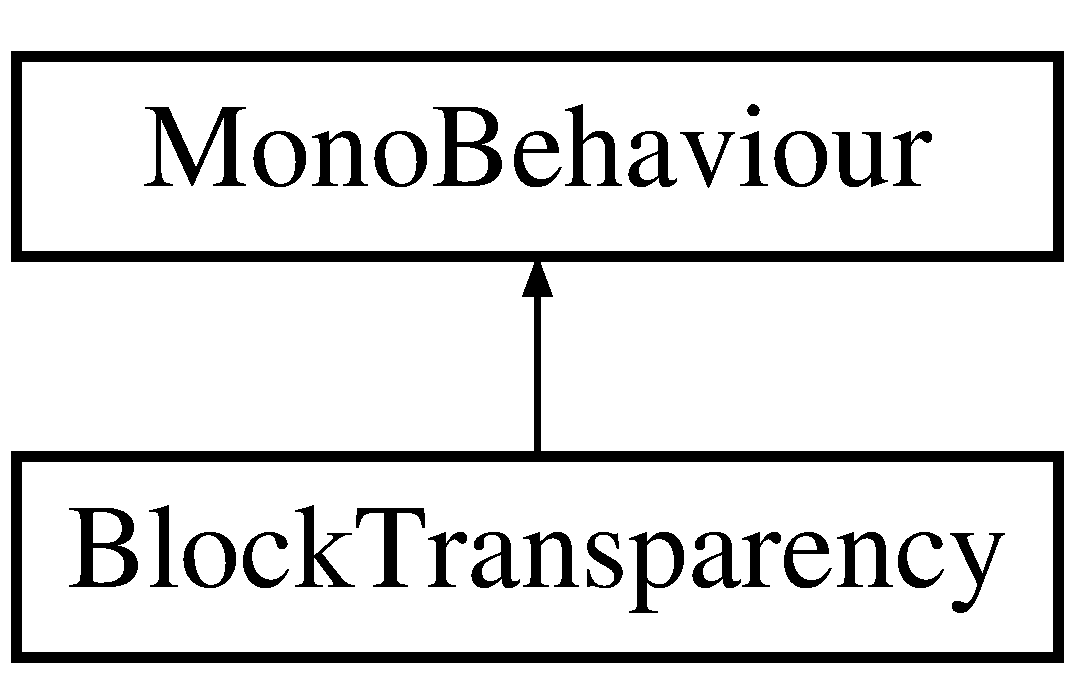
\includegraphics[height=2.000000cm]{class_block_transparency}
\end{center}
\end{figure}
\subsection*{Public Attributes}
\begin{DoxyCompactItemize}
\item 
\hypertarget{class_block_transparency_a7c5f9720e40e90ec89cd73ef14ee6623}{Game\+Object {\bfseries player}}\label{class_block_transparency_a7c5f9720e40e90ec89cd73ef14ee6623}

\item 
\hypertarget{class_block_transparency_a3911a87b05cf6726d9b75c5d528ae958}{float {\bfseries distance\+Till\+Fade} = 2.\+5f}\label{class_block_transparency_a3911a87b05cf6726d9b75c5d528ae958}

\end{DoxyCompactItemize}


\subsection{Detailed Description}
This component allows for transparent transition of a Game\+Object if some other collider is nearby. In this case the Player. 



Definition at line 7 of file Block\+Transparency.\+cs.



The documentation for this class was generated from the following file\+:\begin{DoxyCompactItemize}
\item 
Assets/\+Scripts/\+Level\+Scripts/Block\+Transparency.\+cs\end{DoxyCompactItemize}

\hypertarget{class_drop_block}{\section{Drop\+Block Class Reference}
\label{class_drop_block}\index{Drop\+Block@{Drop\+Block}}
}


Component used to ease a levelpart downwards. Controlled in the editor by Drop\+Block\+Helper  


Inheritance diagram for Drop\+Block\+:\begin{figure}[H]
\begin{center}
\leavevmode
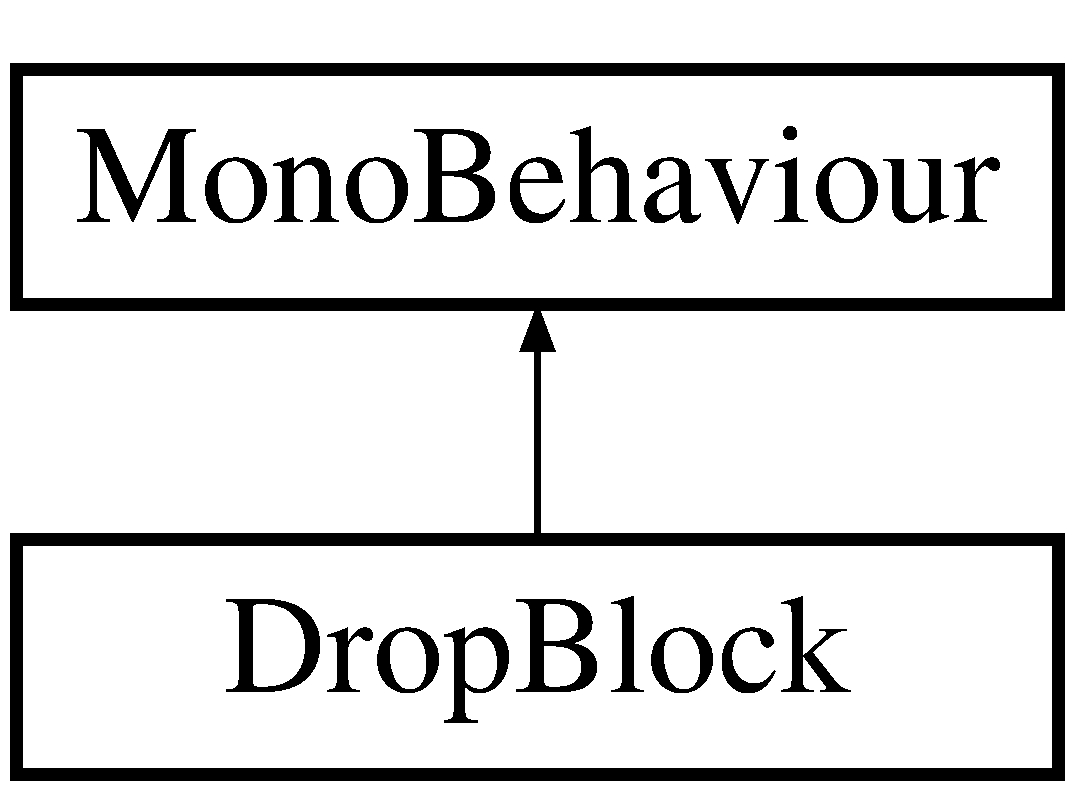
\includegraphics[height=2.000000cm]{class_drop_block}
\end{center}
\end{figure}


\subsection{Detailed Description}
Component used to ease a levelpart downwards. Controlled in the editor by Drop\+Block\+Helper 



Definition at line 7 of file Drop\+Block.\+cs.



The documentation for this class was generated from the following file\+:\begin{DoxyCompactItemize}
\item 
Assets/\+Scripts/\+Level\+Scripts/Drop\+Block.\+cs\end{DoxyCompactItemize}

\hypertarget{class_drop_borders}{\section{Drop\+Borders Class Reference}
\label{class_drop_borders}\index{Drop\+Borders@{Drop\+Borders}}
}


This component lowers or raises the borders as one object. This component is dependent on \hyperlink{class_drop_block}{Drop\+Block}'s interaction with the player.  


Inheritance diagram for Drop\+Borders\+:\begin{figure}[H]
\begin{center}
\leavevmode
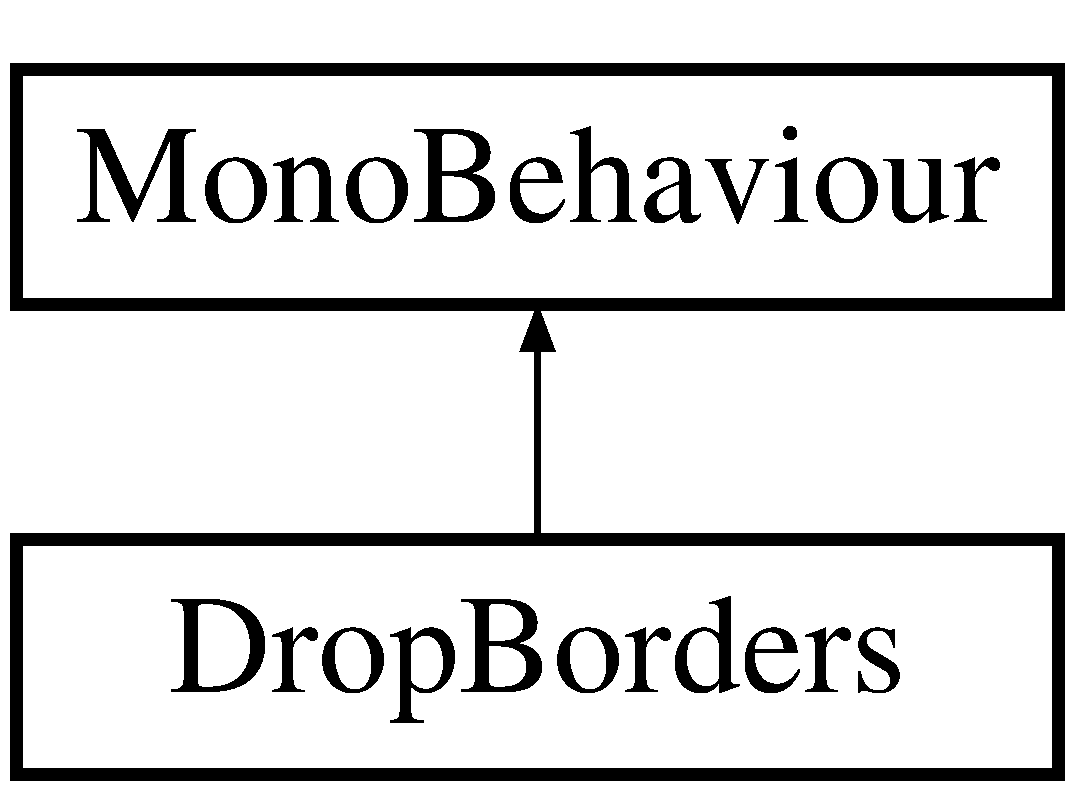
\includegraphics[height=2.000000cm]{class_drop_borders}
\end{center}
\end{figure}
\subsection*{Public Member Functions}
\begin{DoxyCompactItemize}
\item 
\hypertarget{class_drop_borders_a496db05538c10dddd1399bd77bb8f11d}{void {\bfseries Set\+Lift\+Values} (float time)}\label{class_drop_borders_a496db05538c10dddd1399bd77bb8f11d}

\item 
\hypertarget{class_drop_borders_a4d6ea1934875e48ed596c77c7df768a9}{void {\bfseries Lift\+Blocks} ()}\label{class_drop_borders_a4d6ea1934875e48ed596c77c7df768a9}

\end{DoxyCompactItemize}
\subsection*{Public Attributes}
\begin{DoxyCompactItemize}
\item 
\hypertarget{class_drop_borders_a50655a57d9e07d963714c063a423e7f4}{float {\bfseries lift\+Duration} = 1.\+61803f}\label{class_drop_borders_a50655a57d9e07d963714c063a423e7f4}

\item 
\hypertarget{class_drop_borders_ac010c9e198f3c259aed9eb5c528497bf}{Signal\+Plan {\bfseries signal\+Plan}}\label{class_drop_borders_ac010c9e198f3c259aed9eb5c528497bf}

\end{DoxyCompactItemize}


\subsection{Detailed Description}
This component lowers or raises the borders as one object. This component is dependent on \hyperlink{class_drop_block}{Drop\+Block}'s interaction with the player. 



Definition at line 14 of file Drop\+Borders.\+cs.



The documentation for this class was generated from the following file\+:\begin{DoxyCompactItemize}
\item 
Assets/\+Scripts/\+Level\+Scripts/Drop\+Borders.\+cs\end{DoxyCompactItemize}

\hypertarget{class_follow_player}{\section{Follow\+Player Class Reference}
\label{class_follow_player}\index{Follow\+Player@{Follow\+Player}}
}


This component ensures the Camera follows the player. The player\+Object is checked for an active instane as well.  


Inheritance diagram for Follow\+Player\+:\begin{figure}[H]
\begin{center}
\leavevmode
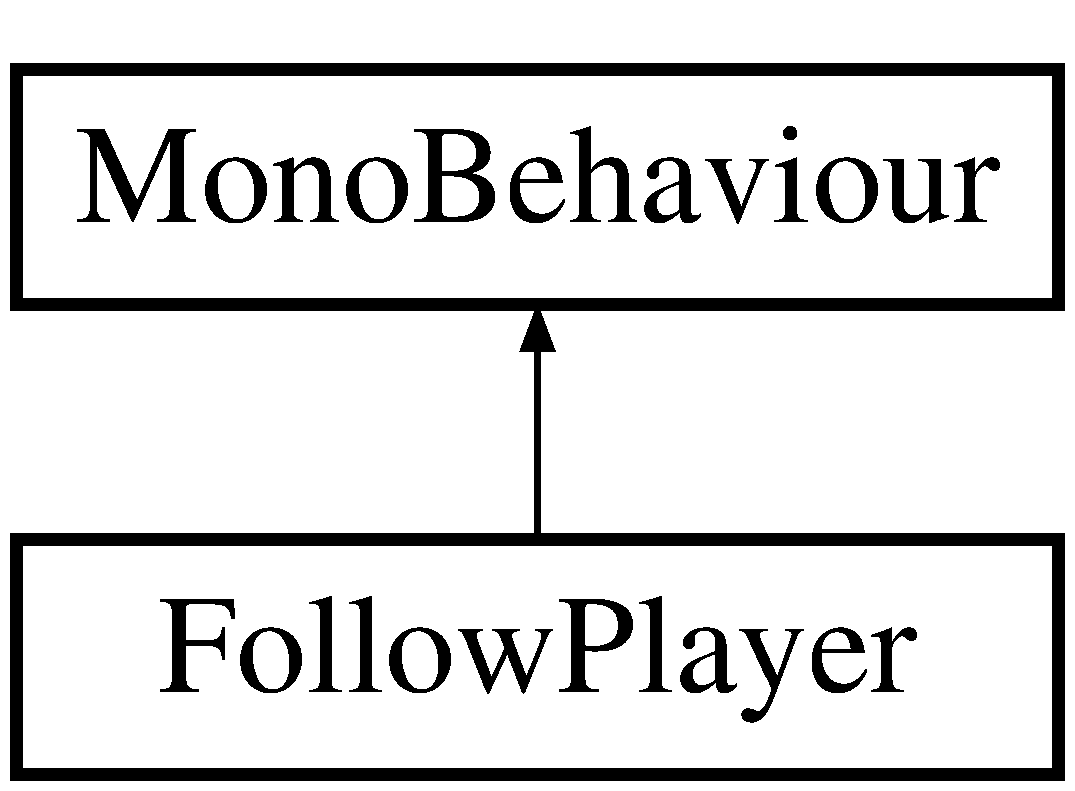
\includegraphics[height=2.000000cm]{class_follow_player}
\end{center}
\end{figure}
\subsection*{Public Attributes}
\begin{DoxyCompactItemize}
\item 
\hypertarget{class_follow_player_a9e8f8c2056e1c3e3dd80d14536adabcd}{Game\+Object {\bfseries player\+Object}}\label{class_follow_player_a9e8f8c2056e1c3e3dd80d14536adabcd}

\end{DoxyCompactItemize}


\subsection{Detailed Description}
This component ensures the Camera follows the player. The player\+Object is checked for an active instane as well. 



Definition at line 7 of file Follow\+Player.\+cs.



The documentation for this class was generated from the following file\+:\begin{DoxyCompactItemize}
\item 
Assets/\+Scripts/\+Player\+Scripts/Follow\+Player.\+cs\end{DoxyCompactItemize}

\hypertarget{class_game_config}{\section{Game\+Config Class Reference}
\label{class_game_config}\index{Game\+Config@{Game\+Config}}
}


Configuration for the game. For use with Get\+Component$<$$>$(); Controlled in the editor by Game\+Config\+Helper  


Inheritance diagram for Game\+Config\+:\begin{figure}[H]
\begin{center}
\leavevmode
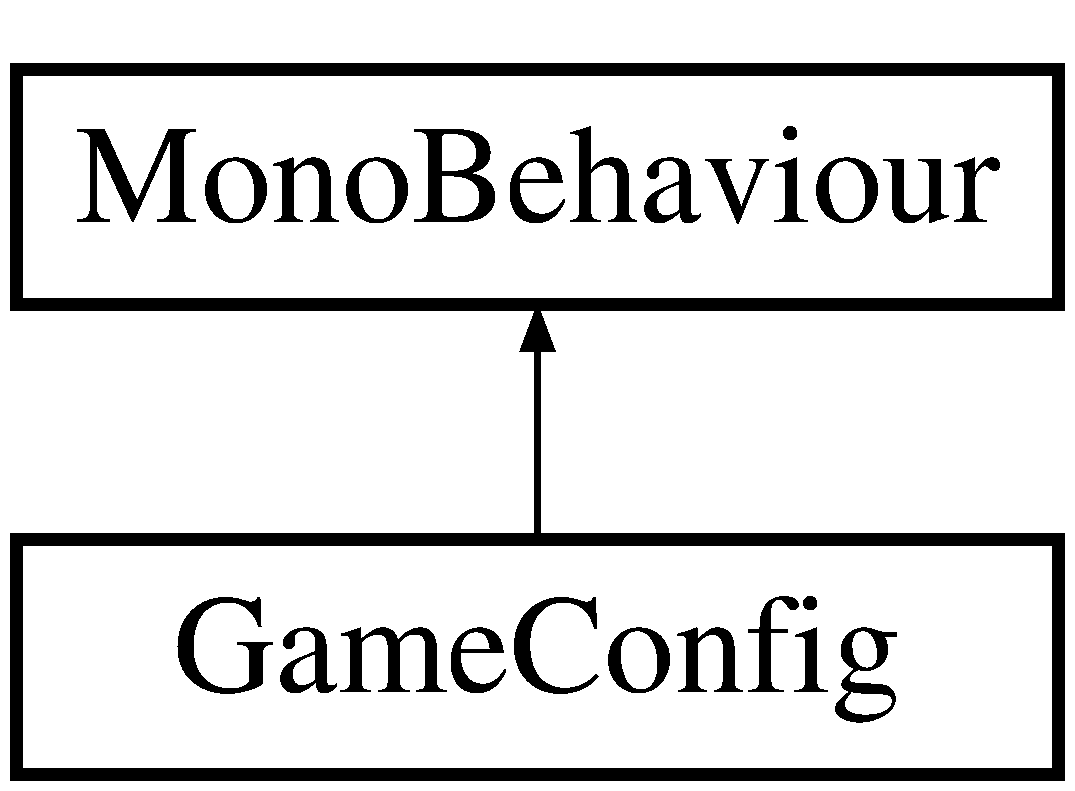
\includegraphics[height=2.000000cm]{class_game_config}
\end{center}
\end{figure}
\subsection*{Public Attributes}
\begin{DoxyCompactItemize}
\item 
\hypertarget{class_game_config_a7ff8b994fa969ec37d290f5417e9f668}{string {\bfseries level\+Name} = \char`\"{}Level01\char`\"{}}\label{class_game_config_a7ff8b994fa969ec37d290f5417e9f668}

\item 
\hypertarget{class_game_config_a57453d5451afd7d19e541567385a5e24}{float {\bfseries player\+Speed} = 1.\+61803f}\label{class_game_config_a57453d5451afd7d19e541567385a5e24}

\item 
\hypertarget{class_game_config_ac61c80bdbd45f3fc7dc1a0e71bb993be}{int {\bfseries pick\+Up\+Coin\+Value} = 10}\label{class_game_config_ac61c80bdbd45f3fc7dc1a0e71bb993be}

\end{DoxyCompactItemize}


\subsection{Detailed Description}
Configuration for the game. For use with Get\+Component$<$$>$(); Controlled in the editor by Game\+Config\+Helper 



Definition at line 8 of file Game\+Config.\+cs.



The documentation for this class was generated from the following file\+:\begin{DoxyCompactItemize}
\item 
Assets/\+Scripts/\+Level\+Scripts/Game\+Config.\+cs\end{DoxyCompactItemize}

\hypertarget{class_high_score_g_u_i}{\section{High\+Score\+G\+U\+I Class Reference}
\label{class_high_score_g_u_i}\index{High\+Score\+G\+U\+I@{High\+Score\+G\+U\+I}}
}


This component manages the score to be displayed properly in the game. It retrieves a player\+Object via Get\+Component$<$$>$(); It also updates the \hyperlink{class_score_counter}{Score\+Counter} with the new score.  


Inheritance diagram for High\+Score\+G\+U\+I\+:\begin{figure}[H]
\begin{center}
\leavevmode
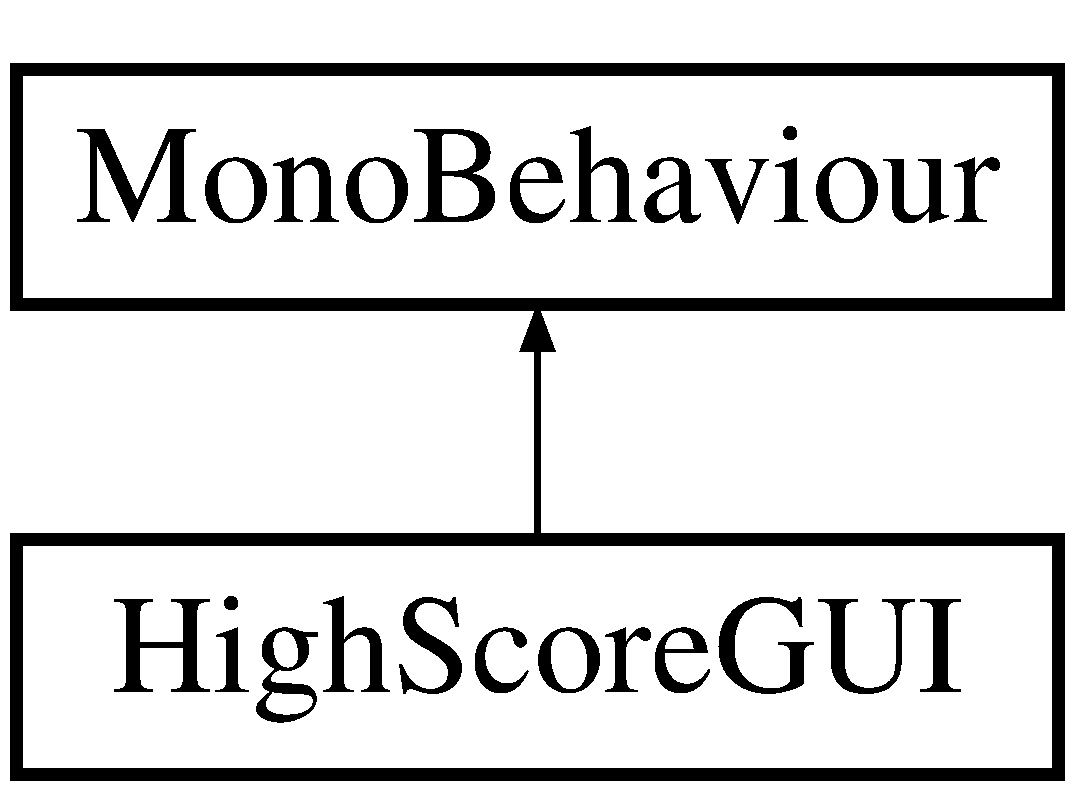
\includegraphics[height=2.000000cm]{class_high_score_g_u_i}
\end{center}
\end{figure}
\subsection*{Public Attributes}
\begin{DoxyCompactItemize}
\item 
\hypertarget{class_high_score_g_u_i_a54ad721c58e2a92affe772079cbfe1e4}{int {\bfseries total\+Points}}\label{class_high_score_g_u_i_a54ad721c58e2a92affe772079cbfe1e4}

\end{DoxyCompactItemize}


\subsection{Detailed Description}
This component manages the score to be displayed properly in the game. It retrieves a player\+Object via Get\+Component$<$$>$(); It also updates the \hyperlink{class_score_counter}{Score\+Counter} with the new score. 



Definition at line 8 of file High\+Score\+G\+U\+I.\+cs.



The documentation for this class was generated from the following file\+:\begin{DoxyCompactItemize}
\item 
Assets/\+Scripts/\+U\+I/High\+Score\+G\+U\+I.\+cs\end{DoxyCompactItemize}

\hypertarget{class_instantiate_game}{\section{Instantiate\+Game Class Reference}
\label{class_instantiate_game}\index{Instantiate\+Game@{Instantiate\+Game}}
}


This component is responsible for loading and instantiating objects needed for the game. 
\begin{DoxyParams}{Parameters}
{\em player} & The prefab/\+Game\+Object controlled by the player\\
\hline
{\em level} & The switchable level, switchable by setting 'level\+Name'\\
\hline
{\em playing\+Field\+Volume} & The box collider to aid in 'respawning' the player by setting the proper\\
\hline
\end{DoxyParams}
 


Inheritance diagram for Instantiate\+Game\+:\begin{figure}[H]
\begin{center}
\leavevmode
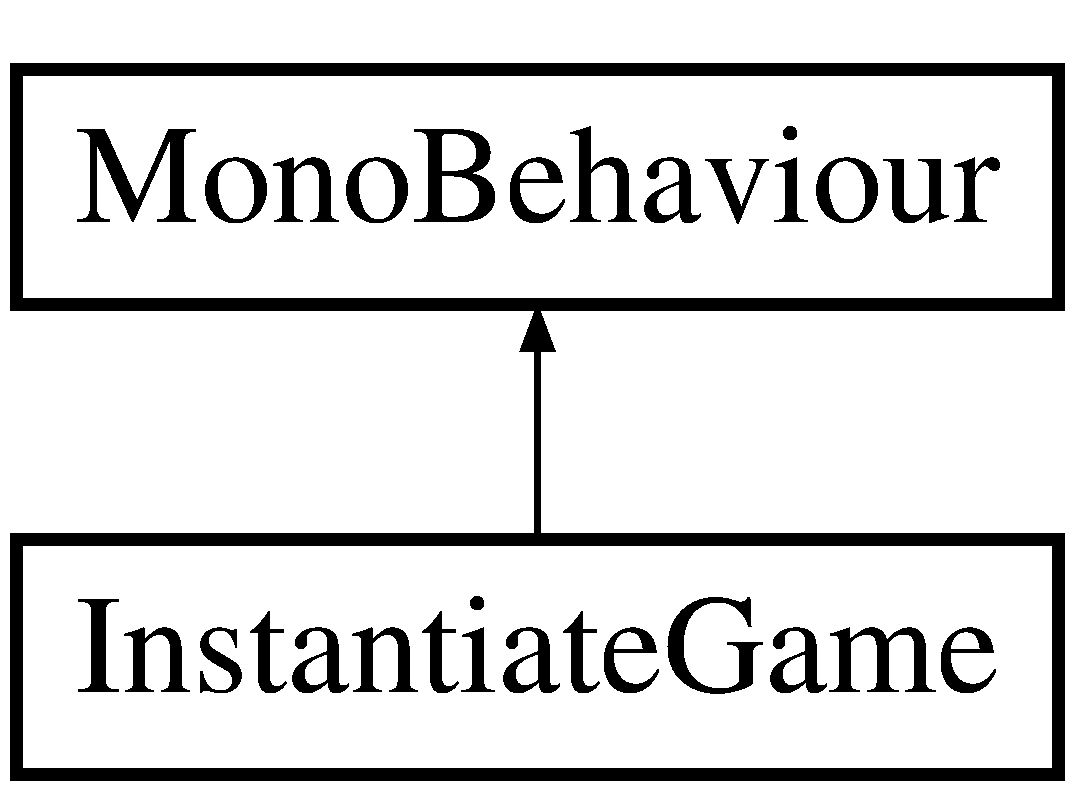
\includegraphics[height=2.000000cm]{class_instantiate_game}
\end{center}
\end{figure}
\subsection*{Public Attributes}
\begin{DoxyCompactItemize}
\item 
\hypertarget{class_instantiate_game_a8ac0d43647e0986b73960158303b0bb9}{Game\+Object {\bfseries game\+Config\+Object}}\label{class_instantiate_game_a8ac0d43647e0986b73960158303b0bb9}

\end{DoxyCompactItemize}


\subsection{Detailed Description}
This component is responsible for loading and instantiating objects needed for the game. 
\begin{DoxyParams}{Parameters}
{\em player} & The prefab/\+Game\+Object controlled by the player\\
\hline
{\em level} & The switchable level, switchable by setting 'level\+Name'\\
\hline
{\em playing\+Field\+Volume} & The box collider to aid in 'respawning' the player by setting the proper\\
\hline
\end{DoxyParams}




Definition at line 11 of file Instantiate\+Game.\+cs.



The documentation for this class was generated from the following file\+:\begin{DoxyCompactItemize}
\item 
Assets/\+Scripts/\+Level\+Scripts/Instantiate\+Game.\+cs\end{DoxyCompactItemize}

\hypertarget{class_pause_conditions}{\section{Pause\+Conditions Class Reference}
\label{class_pause_conditions}\index{Pause\+Conditions@{Pause\+Conditions}}
}


This component allows the game to pause if the players are not playing the game properly or if they want to take a break. Or if the supervising mentor wants to intervene.  


Inheritance diagram for Pause\+Conditions\+:\begin{figure}[H]
\begin{center}
\leavevmode
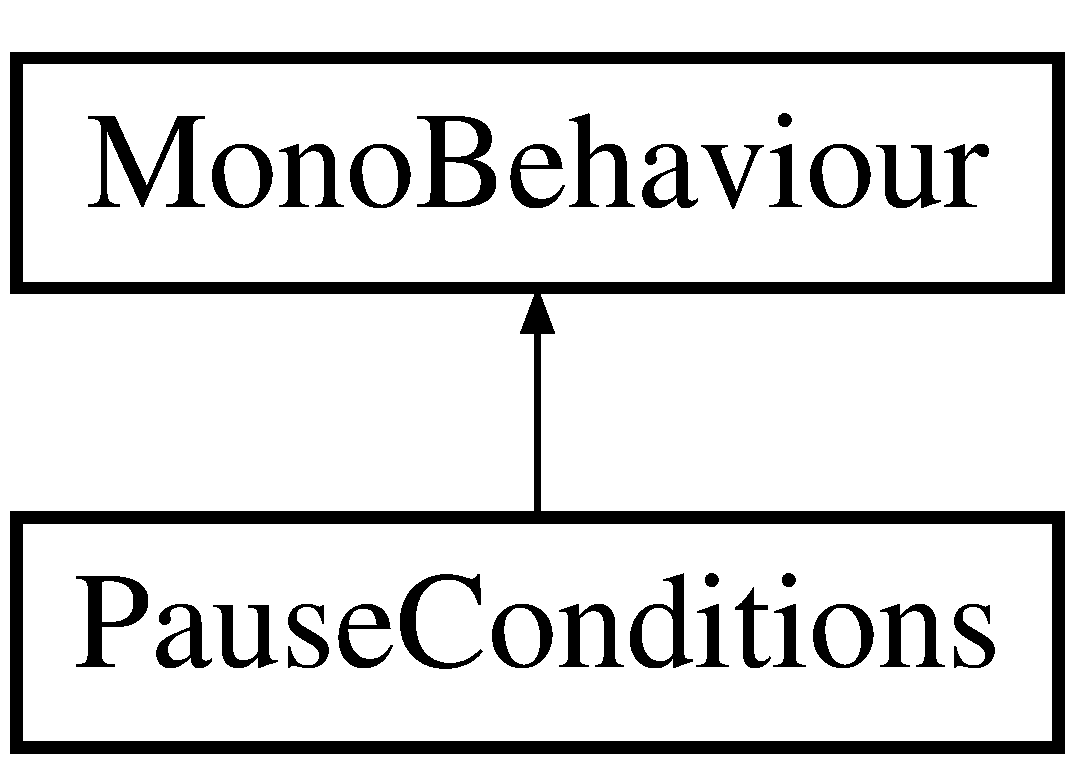
\includegraphics[height=2.000000cm]{class_pause_conditions}
\end{center}
\end{figure}
\subsection*{Public Attributes}
\begin{DoxyCompactItemize}
\item 
\hypertarget{class_pause_conditions_a7f54bf5a4189e3d26bbc97a1e2854e63}{Game\+Object {\bfseries button1}}\label{class_pause_conditions_a7f54bf5a4189e3d26bbc97a1e2854e63}

\item 
\hypertarget{class_pause_conditions_a04ca1e5c5090211701027657bb00980d}{Game\+Object {\bfseries button2}}\label{class_pause_conditions_a04ca1e5c5090211701027657bb00980d}

\item 
\hypertarget{class_pause_conditions_abe537000890aabbfa050bfa63890fd13}{Game\+Object {\bfseries button3}}\label{class_pause_conditions_abe537000890aabbfa050bfa63890fd13}

\item 
\hypertarget{class_pause_conditions_a0a07c7c652aedc49d722d046bec5ae4c}{Game\+Object {\bfseries button4}}\label{class_pause_conditions_a0a07c7c652aedc49d722d046bec5ae4c}

\item 
\hypertarget{class_pause_conditions_aa4c6398400a160dc567f2aa5c146631a}{string {\bfseries button\+State} = \char`\"{}up\char`\"{}}\label{class_pause_conditions_aa4c6398400a160dc567f2aa5c146631a}

\end{DoxyCompactItemize}


\subsection{Detailed Description}
This component allows the game to pause if the players are not playing the game properly or if they want to take a break. Or if the supervising mentor wants to intervene. 



Definition at line 7 of file Pause\+Conditions.\+cs.



The documentation for this class was generated from the following file\+:\begin{DoxyCompactItemize}
\item 
Assets/\+Scripts/\+U\+I/Pause\+Conditions.\+cs\end{DoxyCompactItemize}

\hypertarget{class_pickup_coin}{\section{Pickup\+Coin Class Reference}
\label{class_pickup_coin}\index{Pickup\+Coin@{Pickup\+Coin}}
}
Inheritance diagram for Pickup\+Coin\+:\begin{figure}[H]
\begin{center}
\leavevmode
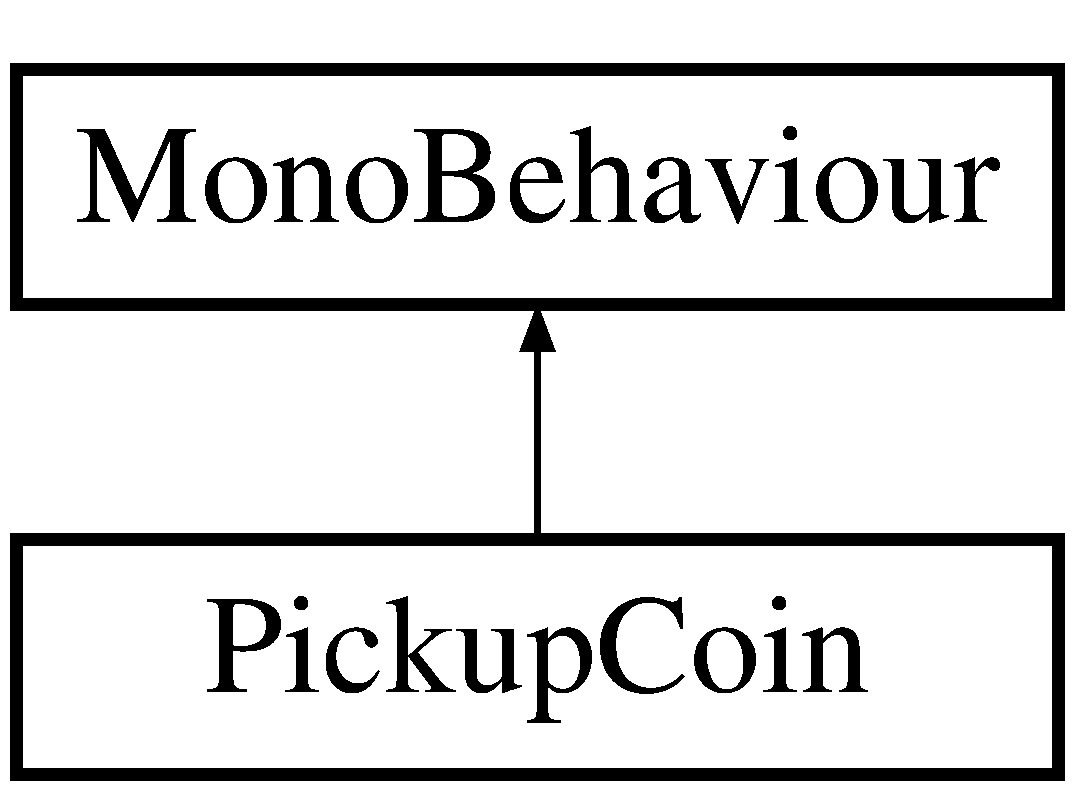
\includegraphics[height=2.000000cm]{class_pickup_coin}
\end{center}
\end{figure}


\subsection{Detailed Description}


Definition at line 4 of file Pickup\+Coin.\+cs.



The documentation for this class was generated from the following file\+:\begin{DoxyCompactItemize}
\item 
Assets/\+Scripts/\+Level\+Scripts/Pickup\+Coin.\+cs\end{DoxyCompactItemize}

\hypertarget{class_reset_player}{\section{Reset\+Player Class Reference}
\label{class_reset_player}\index{Reset\+Player@{Reset\+Player}}
}


This component ensures the level resets the player.  


Inheritance diagram for Reset\+Player\+:\begin{figure}[H]
\begin{center}
\leavevmode
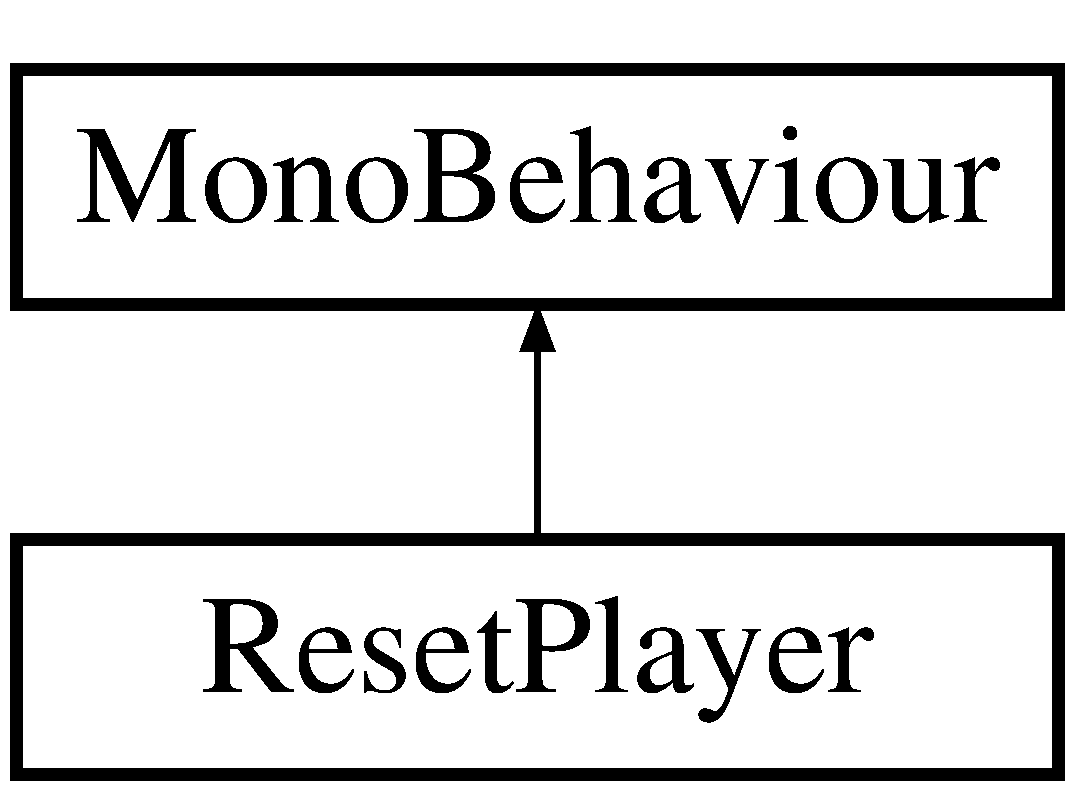
\includegraphics[height=2.000000cm]{class_reset_player}
\end{center}
\end{figure}


\subsection{Detailed Description}
This component ensures the level resets the player. 



Definition at line 6 of file Reset\+Player.\+cs.



The documentation for this class was generated from the following file\+:\begin{DoxyCompactItemize}
\item 
Assets/\+Scripts/\+Player\+Scripts/Reset\+Player.\+cs\end{DoxyCompactItemize}

\hypertarget{class_rotate_g_u_i}{\section{Rotate\+G\+U\+I Class Reference}
\label{class_rotate_g_u_i}\index{Rotate\+G\+U\+I@{Rotate\+G\+U\+I}}
}
Inheritance diagram for Rotate\+G\+U\+I\+:\begin{figure}[H]
\begin{center}
\leavevmode
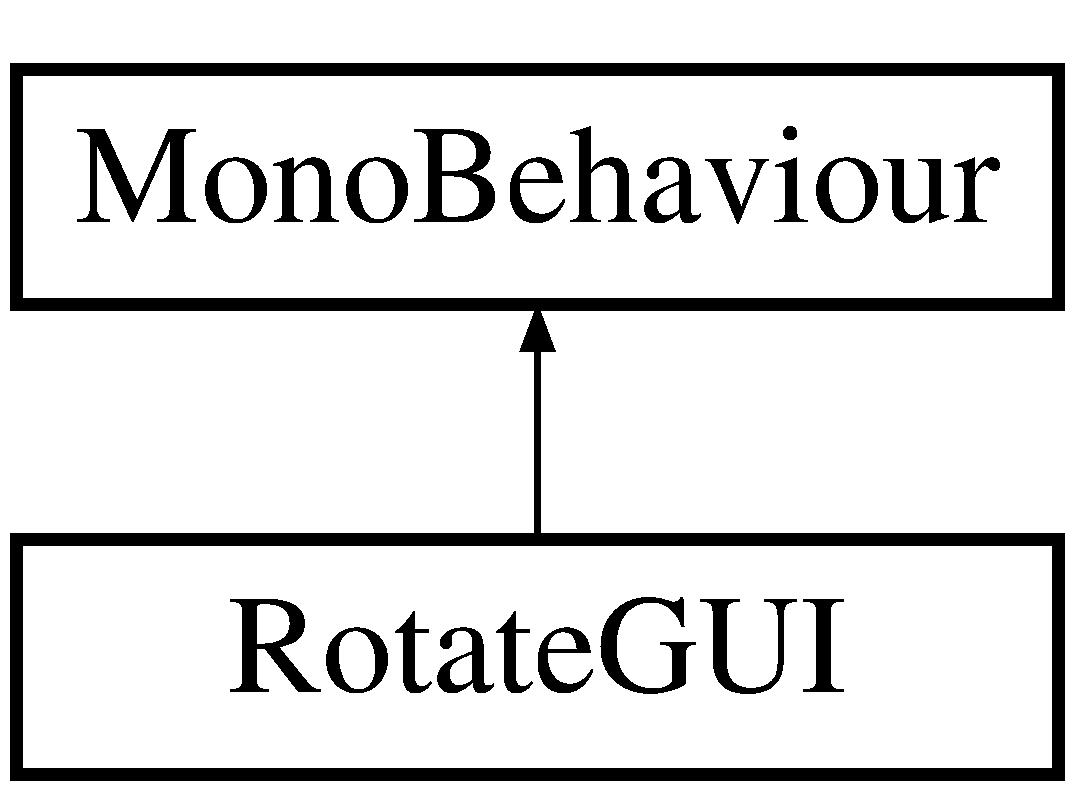
\includegraphics[height=2.000000cm]{class_rotate_g_u_i}
\end{center}
\end{figure}
\subsection*{Public Member Functions}
\begin{DoxyCompactItemize}
\item 
\hypertarget{class_rotate_g_u_i_ae8e7588323f5a87a6bf5bf17aa467a9c}{{\bfseries Rotate\+G\+U\+I} (Game\+Object gameobj)}\label{class_rotate_g_u_i_ae8e7588323f5a87a6bf5bf17aa467a9c}

\end{DoxyCompactItemize}
\subsection*{Public Attributes}
\begin{DoxyCompactItemize}
\item 
\hypertarget{class_rotate_g_u_i_a99ba2952cb01bdf28171f04f3f339683}{Texture2\+D {\bfseries texture} = null}\label{class_rotate_g_u_i_a99ba2952cb01bdf28171f04f3f339683}

\item 
\hypertarget{class_rotate_g_u_i_a018bfaff1e804ba93d39c81b142f2f6b}{float {\bfseries angle} = 0}\label{class_rotate_g_u_i_a018bfaff1e804ba93d39c81b142f2f6b}

\item 
\hypertarget{class_rotate_g_u_i_a75558c35bc8468bcbb21fcb488a5de4a}{Vector2 {\bfseries size} = new Vector2(128, 128)}\label{class_rotate_g_u_i_a75558c35bc8468bcbb21fcb488a5de4a}

\end{DoxyCompactItemize}


\subsection{Detailed Description}


Definition at line 4 of file Rotate\+G\+U\+I.\+cs.



The documentation for this class was generated from the following file\+:\begin{DoxyCompactItemize}
\item 
Assets/\+Scripts/\+U\+I/Rotate\+G\+U\+I.\+cs\end{DoxyCompactItemize}

\hypertarget{class_scale_in_game_g_u_i}{\section{Scale\+In\+Game\+G\+U\+I Class Reference}
\label{class_scale_in_game_g_u_i}\index{Scale\+In\+Game\+G\+U\+I@{Scale\+In\+Game\+G\+U\+I}}
}
Inheritance diagram for Scale\+In\+Game\+G\+U\+I\+:\begin{figure}[H]
\begin{center}
\leavevmode
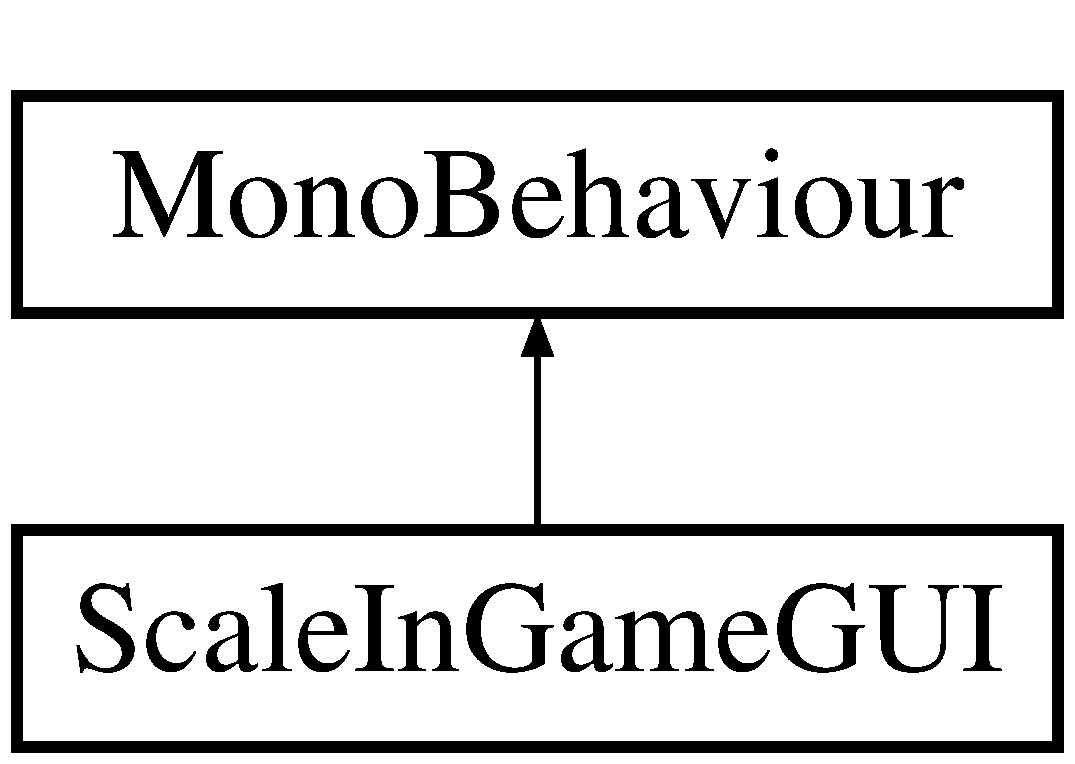
\includegraphics[height=2.000000cm]{class_scale_in_game_g_u_i}
\end{center}
\end{figure}
\subsection*{Public Attributes}
\begin{DoxyCompactItemize}
\item 
\hypertarget{class_scale_in_game_g_u_i_ad1e5aa3fc09488374a71b38602f16f93}{const int {\bfseries calc\+Sizes\+Width} = 720}\label{class_scale_in_game_g_u_i_ad1e5aa3fc09488374a71b38602f16f93}

\item 
\hypertarget{class_scale_in_game_g_u_i_a63c80e42c3125a8b865b812c9e1f5d70}{const int {\bfseries calc\+Sizes\+Height} = 1280}\label{class_scale_in_game_g_u_i_a63c80e42c3125a8b865b812c9e1f5d70}

\end{DoxyCompactItemize}


\subsection{Detailed Description}


Definition at line 4 of file Scale\+In\+Game\+G\+U\+I.\+cs.



The documentation for this class was generated from the following file\+:\begin{DoxyCompactItemize}
\item 
C\+:/\+Projects/\+Unity/\+Proeve van Bekwaamheid/\+Assets/\+Scripts/\+U\+I/Scale\+In\+Game\+G\+U\+I.\+cs\end{DoxyCompactItemize}

\hypertarget{class_score_counter}{\section{Score\+Counter Class Reference}
\label{class_score_counter}\index{Score\+Counter@{Score\+Counter}}
}
Inheritance diagram for Score\+Counter\+:\begin{figure}[H]
\begin{center}
\leavevmode
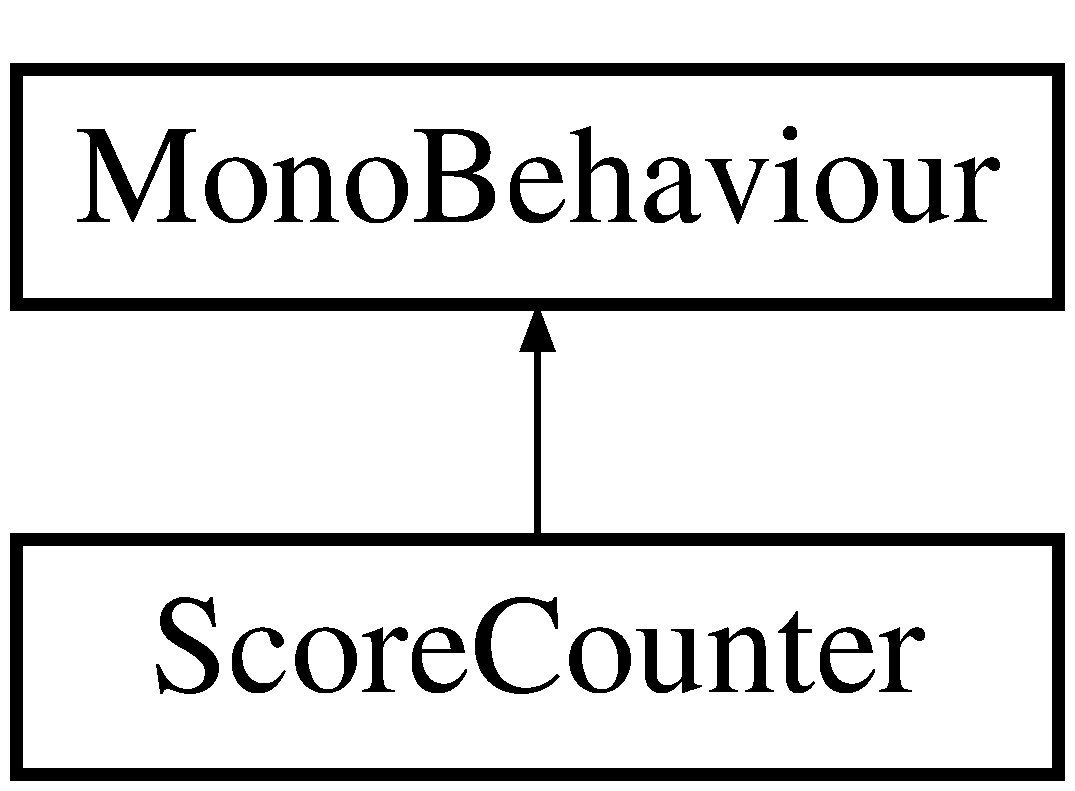
\includegraphics[height=2.000000cm]{class_score_counter}
\end{center}
\end{figure}
\subsection*{Public Attributes}
\begin{DoxyCompactItemize}
\item 
\hypertarget{class_score_counter_a4dfb92a30d6b9f84514a10ebcf138692}{int {\bfseries total\+Points}}\label{class_score_counter_a4dfb92a30d6b9f84514a10ebcf138692}

\end{DoxyCompactItemize}


\subsection{Detailed Description}


Definition at line 4 of file Score\+Counter.\+cs.



The documentation for this class was generated from the following file\+:\begin{DoxyCompactItemize}
\item 
C\+:/\+Projects/\+Unity/\+Proeve van Bekwaamheid/\+Assets/\+Scripts/\+Level\+Scripts/Score\+Counter.\+cs\end{DoxyCompactItemize}

\hypertarget{class_spawn_point}{\section{Spawn\+Point Class Reference}
\label{class_spawn_point}\index{Spawn\+Point@{Spawn\+Point}}
}


Helper class, to store the \hyperlink{class_spawn_point}{Spawn\+Point}. For use with Get\+Component$<$$>$();  


Inheritance diagram for Spawn\+Point\+:\begin{figure}[H]
\begin{center}
\leavevmode
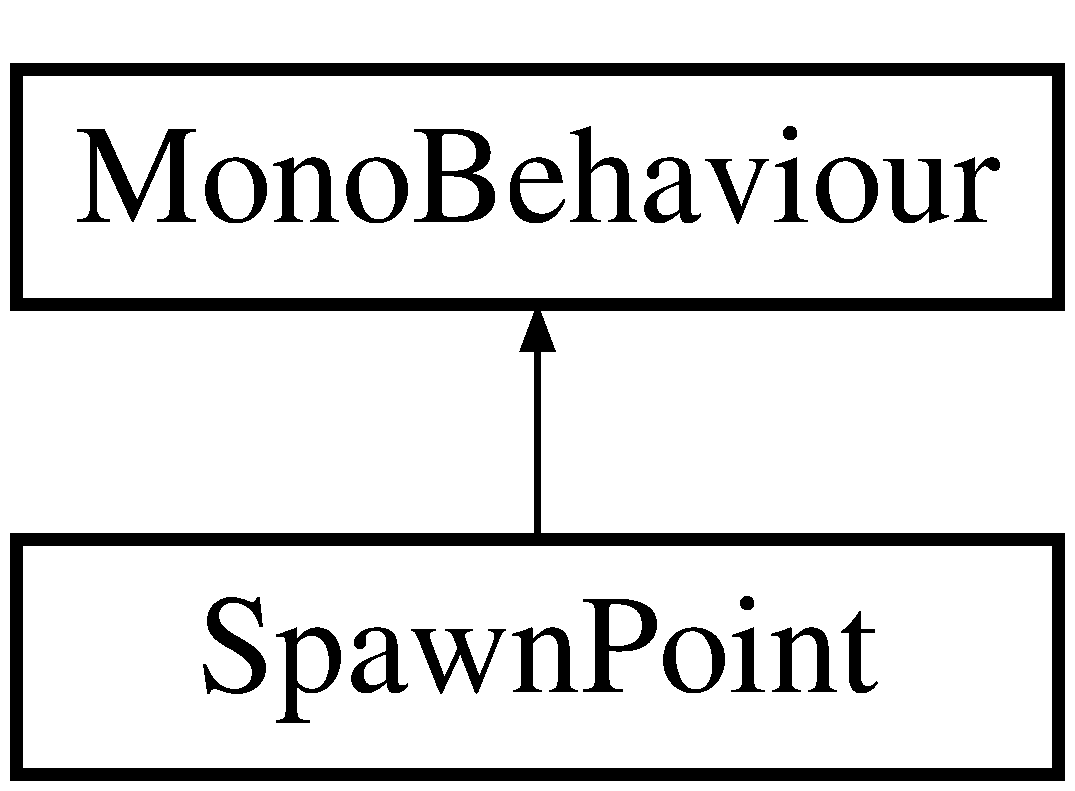
\includegraphics[height=2.000000cm]{class_spawn_point}
\end{center}
\end{figure}
\subsection*{Public Attributes}
\begin{DoxyCompactItemize}
\item 
\hypertarget{class_spawn_point_a1bbcf616b90a7e757535911a313fb838}{Transform {\bfseries spawn\+Point}}\label{class_spawn_point_a1bbcf616b90a7e757535911a313fb838}

\end{DoxyCompactItemize}


\subsection{Detailed Description}
Helper class, to store the \hyperlink{class_spawn_point}{Spawn\+Point}. For use with Get\+Component$<$$>$(); 



Definition at line 7 of file Spawn\+Point.\+cs.



The documentation for this class was generated from the following file\+:\begin{DoxyCompactItemize}
\item 
Assets/\+Scripts/\+Level\+Scripts/Spawn\+Point.\+cs\end{DoxyCompactItemize}

\hypertarget{class_u_i_level_select}{\section{U\+I\+Level\+Select Class Reference}
\label{class_u_i_level_select}\index{U\+I\+Level\+Select@{U\+I\+Level\+Select}}
}
Inheritance diagram for U\+I\+Level\+Select\+:\begin{figure}[H]
\begin{center}
\leavevmode
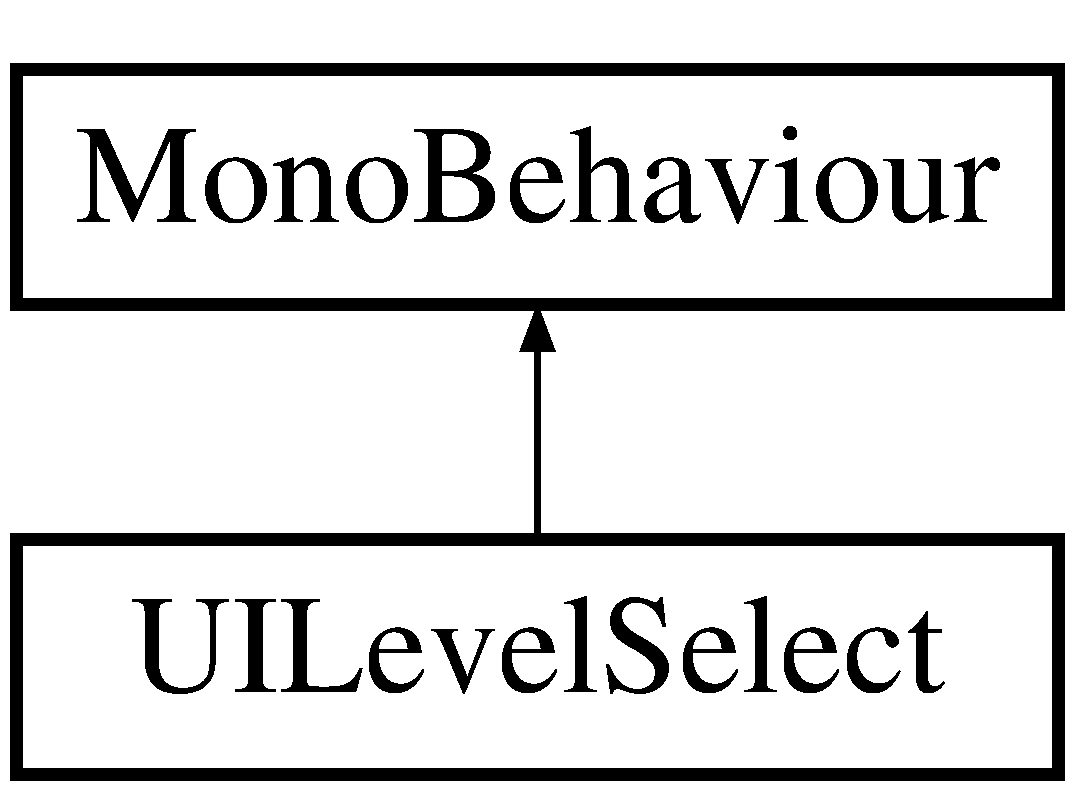
\includegraphics[height=2.000000cm]{class_u_i_level_select}
\end{center}
\end{figure}
\subsection*{Public Attributes}
\begin{DoxyCompactItemize}
\item 
\hypertarget{class_u_i_level_select_a48db57556771bc8772b6dd0d67ca825c}{G\+U\+I\+Style {\bfseries button\+Style}}\label{class_u_i_level_select_a48db57556771bc8772b6dd0d67ca825c}

\item 
\hypertarget{class_u_i_level_select_a1f9a7875be68967a261164156a5a1041}{int {\bfseries level\+Amount} = 10}\label{class_u_i_level_select_a1f9a7875be68967a261164156a5a1041}

\item 
\hypertarget{class_u_i_level_select_a7ec603d5e50e86c260987cde94930ca6}{int {\bfseries column\+Amount} = 3}\label{class_u_i_level_select_a7ec603d5e50e86c260987cde94930ca6}

\item 
\hypertarget{class_u_i_level_select_a73267fc8dd1334e9a2d347d2f9adfcaf}{int {\bfseries padding\+X} = 100}\label{class_u_i_level_select_a73267fc8dd1334e9a2d347d2f9adfcaf}

\item 
\hypertarget{class_u_i_level_select_a1cdd4182fe75a9a9c756bf5585cdb196}{int {\bfseries padding\+Y} = 100}\label{class_u_i_level_select_a1cdd4182fe75a9a9c756bf5585cdb196}

\item 
\hypertarget{class_u_i_level_select_a3306a87ad81b8953e51c3cb2ccf70e3f}{int {\bfseries button\+Width} = 100}\label{class_u_i_level_select_a3306a87ad81b8953e51c3cb2ccf70e3f}

\item 
\hypertarget{class_u_i_level_select_ac6329aeb4188e8e54b468fc0e03d8569}{int {\bfseries button\+Height} = 50}\label{class_u_i_level_select_ac6329aeb4188e8e54b468fc0e03d8569}

\item 
\hypertarget{class_u_i_level_select_ae933076aa310b962df6f38fb4dba90e2}{int {\bfseries starting\+Pos\+Height} = 100}\label{class_u_i_level_select_ae933076aa310b962df6f38fb4dba90e2}

\item 
\hypertarget{class_u_i_level_select_ae85a31e3090795c6dad84b6050e0bbf4}{float {\bfseries set\+Size} = 1}\label{class_u_i_level_select_ae85a31e3090795c6dad84b6050e0bbf4}

\item 
\hypertarget{class_u_i_level_select_a59a1686f78e7d6b01e8e23abadf2123e}{const int {\bfseries calc\+Sizes\+Width} = 1280}\label{class_u_i_level_select_a59a1686f78e7d6b01e8e23abadf2123e}

\item 
\hypertarget{class_u_i_level_select_a18d2c15a8a1ca38c60b94594816742a9}{const int {\bfseries calc\+Sizes\+Height} = 720}\label{class_u_i_level_select_a18d2c15a8a1ca38c60b94594816742a9}

\end{DoxyCompactItemize}


\subsection{Detailed Description}


Definition at line 4 of file U\+I\+Level\+Select.\+cs.



The documentation for this class was generated from the following file\+:\begin{DoxyCompactItemize}
\item 
C\+:/\+Projects/\+Unity/\+Proeve van Bekwaamheid/\+Assets/\+Scripts/\+U\+I/U\+I\+Level\+Select.\+cs\end{DoxyCompactItemize}

\hypertarget{class_water_transparency}{\section{Water\+Transparency Class Reference}
\label{class_water_transparency}\index{Water\+Transparency@{Water\+Transparency}}
}


This component allows for transparent transition of a Game\+Object if some other collider is nearby. In this case the Player.  


Inheritance diagram for Water\+Transparency\+:\begin{figure}[H]
\begin{center}
\leavevmode
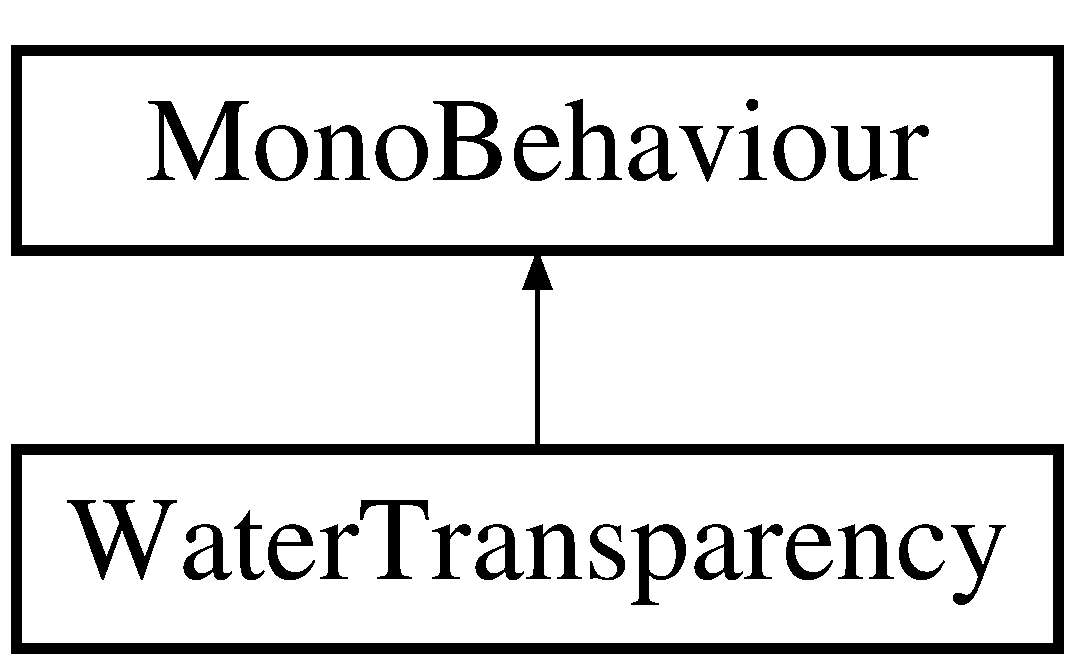
\includegraphics[height=2.000000cm]{class_water_transparency}
\end{center}
\end{figure}
\subsection*{Public Attributes}
\begin{DoxyCompactItemize}
\item 
\hypertarget{class_water_transparency_ac96cfbea16b8832ac2ac3ca56aada830}{Game\+Object {\bfseries player}}\label{class_water_transparency_ac96cfbea16b8832ac2ac3ca56aada830}

\item 
\hypertarget{class_water_transparency_a4b2b69526abb0b842ed31bef14e236f0}{bool {\bfseries change}}\label{class_water_transparency_a4b2b69526abb0b842ed31bef14e236f0}

\end{DoxyCompactItemize}


\subsection{Detailed Description}
This component allows for transparent transition of a Game\+Object if some other collider is nearby. In this case the Player. 



Definition at line 7 of file Water\+Transparency.\+cs.



The documentation for this class was generated from the following file\+:\begin{DoxyCompactItemize}
\item 
C\+:/\+Projects/\+Unity/\+Proeve van Bekwaamheid/\+Assets/\+Scripts/\+Level\+Scripts/Water\+Transparency.\+cs\end{DoxyCompactItemize}

\hypertarget{class_water_trigger}{\section{Water\+Trigger Class Reference}
\label{class_water_trigger}\index{Water\+Trigger@{Water\+Trigger}}
}
Inheritance diagram for Water\+Trigger\+:\begin{figure}[H]
\begin{center}
\leavevmode
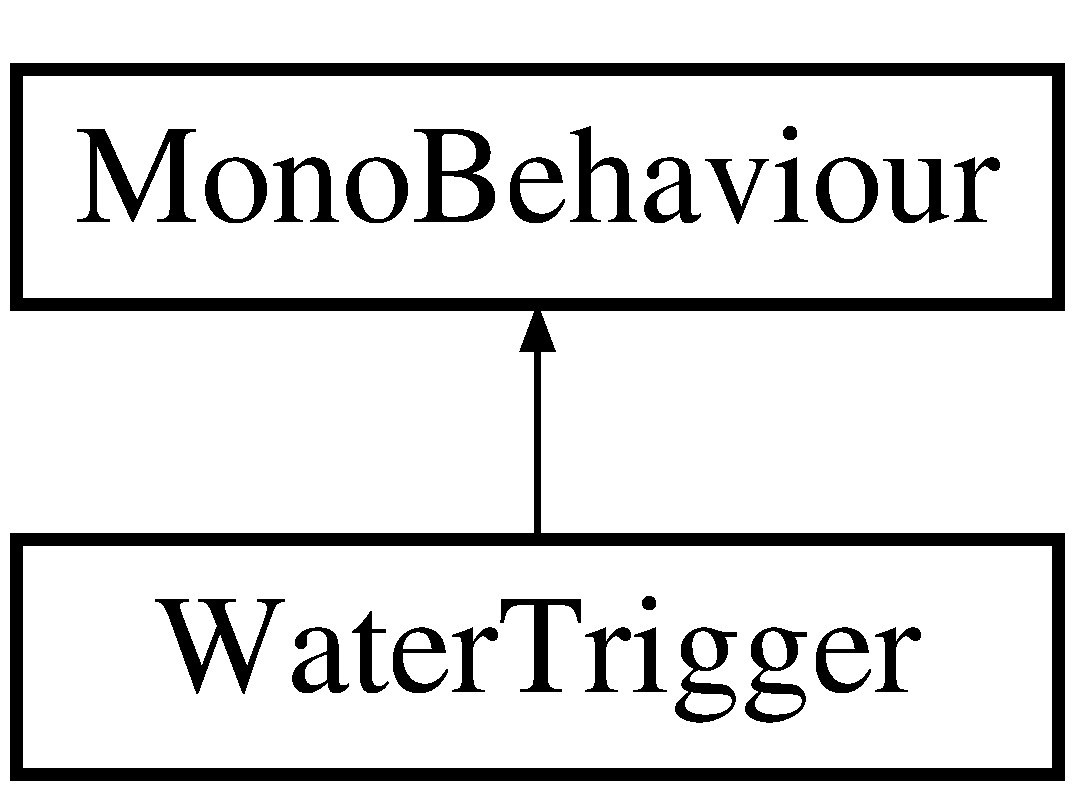
\includegraphics[height=2.000000cm]{class_water_trigger}
\end{center}
\end{figure}


\subsection{Detailed Description}


Definition at line 4 of file Water\+Trigger.\+cs.



The documentation for this class was generated from the following file\+:\begin{DoxyCompactItemize}
\item 
C\+:/\+Projects/\+Unity/\+Proeve van Bekwaamheid/\+Assets/\+Scripts/\+Level\+Scripts/Water\+Trigger.\+cs\end{DoxyCompactItemize}

%--- End generated contents ---

% Index
\newpage
\phantomsection
\addcontentsline{toc}{chapter}{Index}
\printindex

\end{document}
